\documentclass[tikz]{standalone}
\usepackage{tkz-graph}
\usepackage{amsmath,amssymb}
\usepackage{xcolor}
\usetikzlibrary{calc}
\usetikzlibrary{positioning}
\usetikzlibrary{trees}

\begin{document}
% https://latexdraw.com/draw-trees-in-tikz/
\begin{tikzpicture}

	\node {parent}[grow = up]
	child [red]{node {child 1} edge from parent  [dashed]}
	child {node [red] {child 2} edge from parent [blue] node [right, brown]{x}};


	\node at (2,0) {o} [grow=north east]
	child {[fill] circle (2pt)}
	child {[fill] circle (2pt)};

	\node at (4, 0) {x} [grow=300] child {node {a}}
	child {node {b}};

\end{tikzpicture}


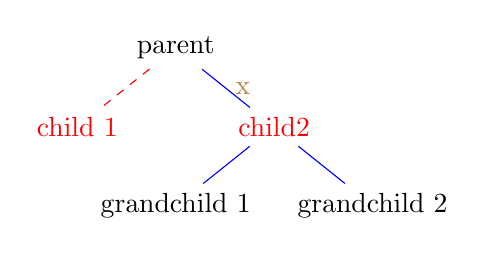
\begin{tikzpicture}
	\node {parent}[sibling distance =2.5cm, level distance = 1cm]
	child [red] {node {child 1} edge from parent [dashed]}
	child {node [red] {child2}
			child {node {grandchild 1}}
			child {node {grandchild 2}}
			edge from parent [blue] node [right, brown]{x}};
\end{tikzpicture}


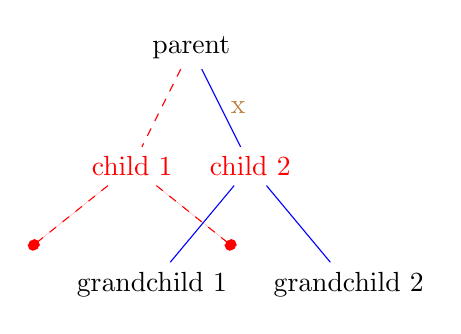
\begin{tikzpicture}

	\node {parent}
	child [red] {node {child 1} [sibling distance = 2.5cm, level distance = 1cm]
			child {[fill] circle (2pt)}
			child {[fill] circle (2pt)}
			edge from parent [dashed]}
	child {node [red] {child 2}[sibling distance = 2.5cm, ]
			child {node {grandchild 1}}
			child {node {grandchild 2}}
			edge from parent [blue] node [right, brown] {x}};

\end{tikzpicture}


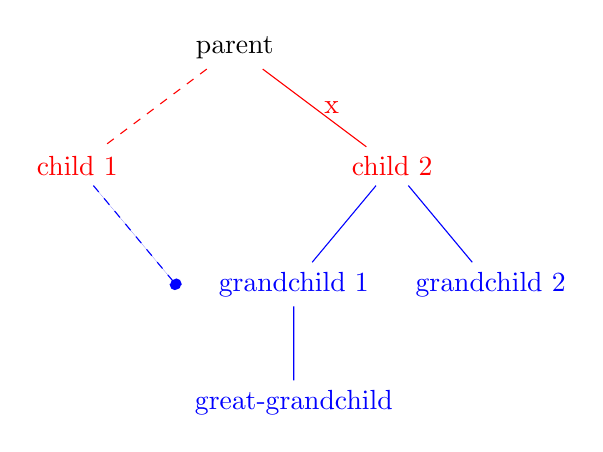
\begin{tikzpicture}
	[
		level 1/.style = {red, sibling distance = 4cm},
		level 2/.style = {blue, sibling distance = 2.5cm}
	]

	\node {parent}
	child {node {child 1}
			child [missing] {[fill] circle (2pt)}
			child {[fill] circle (2pt)}
			edge from parent [dashed]}
	child {node {child 2}
			child {node {grandchild 1}
					child {node {great-grandchild}}}
			child {node {grandchild 2}}
			edge from parent node [right] {x}};

\end{tikzpicture}


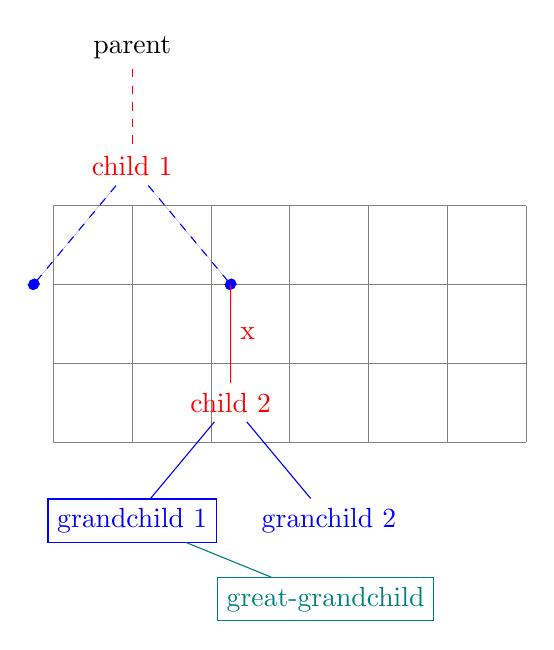
\begin{tikzpicture}
	[
		level 1/.style = {red, sibling distance =4cm},
		level 2/.style = {blue, sibling distance = 2.5cm},
		level 3/.style = {teal, level distance = 1cm},
	]

	\draw [help lines] (-1,-2) grid  (5, -5);
	\node {parent}
	child {node {child 1}
			child {[fill] circle (2pt)}
			child {[fill] circle (2pt)}
			edge from parent [dashed]}

	child {node {child 2}
			child [growth parent anchor= east] {node [draw] {grandchild 1}
					child [anchor= west] {node [draw] {great-grandchild}}}
			child {node {granchild 2}}
			edge from parent node [right] {x}};
\end{tikzpicture}


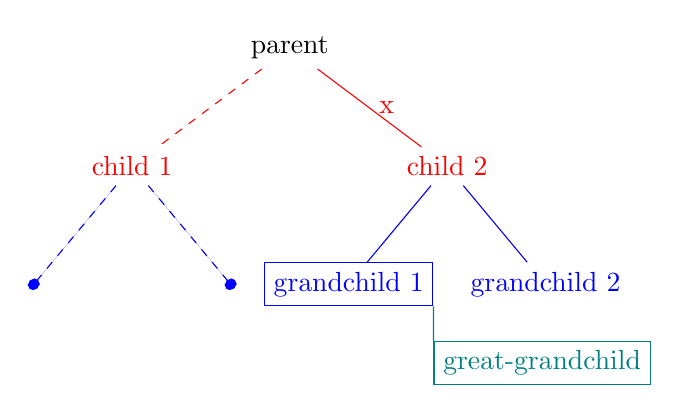
\begin{tikzpicture}[
		level 1/.style = {red, sibling distance = 4cm},
		level 2/.style = {blue, sibling distance = 2.5cm},
		level 3/.style  = {teal, level distance = 1cm}
	]

	\node {parent}
	child {node {child 1}
			child {[fill] circle (2pt)}
			child {[fill] circle (2pt)}
			edge from parent [dashed]}
	child {node {child 2}
			child [growth parent anchor = east] {node [draw] {grandchild 1}
					child [anchor = west,
							parent anchor = south east,
							child anchor = north west] {node [draw] {great-grandchild}}}
			child {node {grandchild 2}}
			edge from parent node [right] {x}};

\end{tikzpicture}



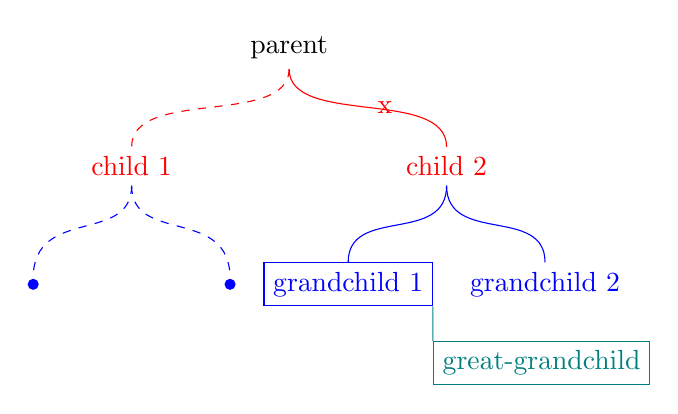
\begin{tikzpicture}[
		level 1/.style  = {red, sibling distance = 4cm},
		level 2/.style = {blue, sibling distance = 2.5cm},
		level 3/.style = {teal, level distance = 1cm},
		edge from parent path =  {(\tikzparentnode\tikzparentanchor) .. controls +(0,-1) and +(0,1) .. (\tikzchildnode\tikzchildanchor)}
	]


	\node {parent}
	child {node {child 1}
			child {node [circle, fill, minimum size = 4pt, inner sep = 0] {}}
			child {node [circle, fill, minimum size = 4pt, inner sep = 0] {}}
			edge from parent [dashed]}
	child {node {child 2}
			child [growth parent anchor = east] {node [draw] {grandchild 1}
					child [anchor = west, parent anchor = south east, child anchor = north west] {node [draw] {great-grandchild}}}
			child {node {grandchild 2}}
			edge from parent node [right] {x}};

\end{tikzpicture}



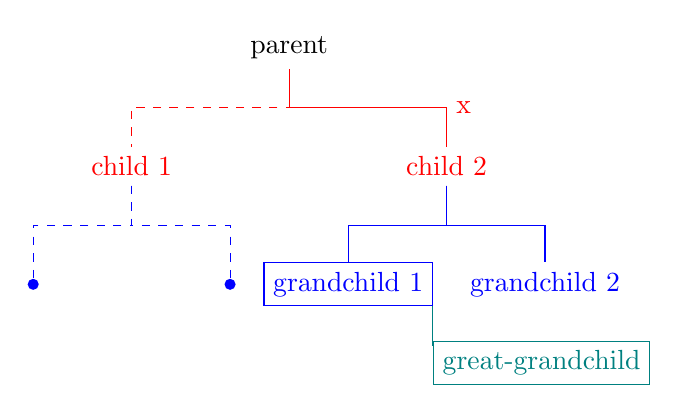
\begin{tikzpicture}
	[
		level 1/.style = {red, sibling distance = 4cm},
		level 2/.style = {blue, sibling distance = 2.5cm},
		level 3/.style = {teal, level distance = 1cm},
		edge from parent fork down
	]

	\node {parent}
	child {node {child 1}
			child {node [circle, fill, minimum size = 4pt, inner sep = 0] {}}
			child {node [circle, fill, minimum size = 4pt, inner sep = 0] {}}
			edge from parent [dashed]}
	child {node {child 2}
			child [growth parent anchor = east] {node [draw] {grandchild 1}
					child [anchor = west, parent anchor = south east, child anchor = north west] {node [draw] {great-grandchild}}}
			child {node {grandchild 2}}
			edge from parent node [right] {x}};

\end{tikzpicture}















\begin{tikzpicture}
	[
		level 1/.style = {red, level distance = 2.5cm, sibling angle = 90},
		level 2/.style = {blue, sibling angle = 60},
		level 3/.style = {teal},
		grow cyclic
	]

	\node {parent}
	child {node {child 1} [clockwise from = 90]
			child {node [circle, fill, minimum size = 4pt, inner sep = 0] {}}
			child {node [circle, fill, minimum size = 4pt, inner sep = 0] {}}
			edge from parent [dashed]}
	child {node {child 2}
			child {node {grandchild 1}
					child {node {great-grandchild}}}
			child {node {grandchild 2}}
			edge from parent node [right] {x}};

\end{tikzpicture}


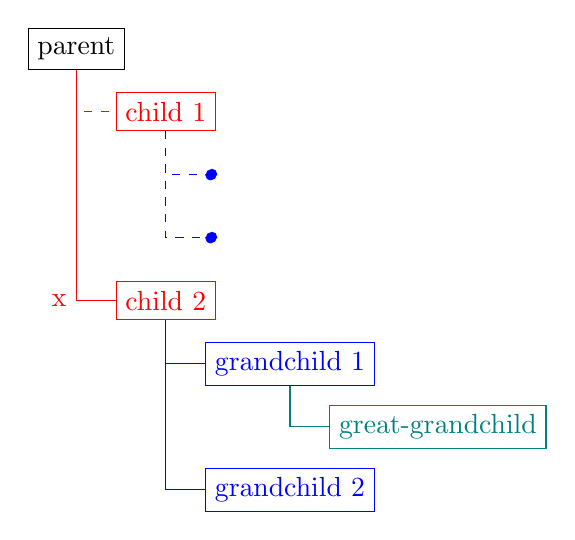
\begin{tikzpicture}
	[
		level 1/.style = {red},
		level 2/.style = {blue},
		level 3/.style = {teal},
		every node/.append style = {draw, anchor = west},
		grow via three points={one child at (0.5,-0.8) and two children at (0.5,-0.8) and (0.5,-1.6)},
		edge from parent path={(\tikzparentnode\tikzparentanchor) |- (\tikzchildnode\tikzchildanchor)}]

	\node {parent}
	child {node {child 1}
			child {node [circle, fill, minimum size = 4pt, inner sep = 0] {}}
			child {node [circle, fill, minimum size = 4pt, inner sep = 0] {}}
			edge from parent [dashed]}
	child [missing] {}
	child [missing] {}
	child {node {child 2}
			child {node {grandchild 1}
					child {node {great-grandchild}}}
			child [missing] {}
			child {node {grandchild 2}}
			edge from parent node [draw = none, left] {x}};

\end{tikzpicture}

\end{document}

